% =====================================================================
% Revision in response to review. Target length: 8 pages.
%
% What changed and why (reviewer point -> response):
%
%  R1.1, R1.4, R2.7  "no novelty vs CEP / rule engines / blackboard"
%      The novelty claim is WITHDRAWN. Section II now positions the system
%      explicitly as a domain instantiation of the rule-engine-over-event-
%      stream pattern and of the ISO 13374 pipeline, with citations, and
%      Table I compares against those rather than against ECAM/EICAS alone.
%      The contribution is restated as empirical, not architectural.
%
%  R1.2, R2.1  "efficiency claims asserted, not measured"
%      Section V replaces the old Scalability section entirely with
%      measurements: per-module cost distribution, aggregate tick latency,
%      deadline-miss rate. Includes the negative result that the
%      architecture's own aggregation stage, not the module population,
%      is the cost driver, and that 0.4% of ticks miss their deadline.
%
%  R1.3, R2.4  "concurrent read/write ordering hazard never addressed"
%      Section VII addresses it directly: why a data race is impossible
%      here, why an ordering hazard is nonetheless real, how large the
%      coupling surface actually is (measured), and that the failure mode
%      is alert suppression.
%
%  R2.2  "no FDR evaluation"
%      Section VIII reports it. All measurements in this revision come from
%      replayed DASHlink FDR recordings, not from the generator. The
%      post-correction figure (33) is re-measured on the current build over
%      the complete 150.8-minute flight that produced the 2,409 baseline.
%
%  R2.3  "re-certification claim overly optimistic"
%      WITHDRAWN. Section X states plainly that nothing here constitutes a
%      certification argument.
%
%  R2.5  "contracts by convention"  R2.6  "naive fusion"
%      Both acknowledged as limitations in Section X, with the eleven
%      convention-violating handlers counted rather than hand-waved, and
%      with the fusion alternatives cited.
%
% ALSO ADDED IN THIS PASS (further reviewer points, previously unanswered):
%
%  R1.2  "no discussion of how the 53 modules were validated against the
%         regulatory limits they claim to encode"
%      Section VIII.C is new and audits it: 133 numeric constants, 7 of 54
%      modules (13%) naming any regulatory source, 113 constants with no
%      recorded origin. The Section III claim about "named published limits"
%      is corrected accordingly rather than left standing.
%
%  R1.2  "no test suite description"
%      Stated plainly in Section VIII.C: there is no automated test suite.
%
%  R1.2  Table II "files modified = 2" is not an experimental result
%      That table is withdrawn; the withdrawal is stated in Section IX.
%
%  R2.1  "CPU/memory overhead, throughput"
%      Section V.D: 860 ticks/s unpaced (54x real time), 1.78% of one core at
%      16 Hz, 119 MB resident, +0.3 MB over 20,000 ticks.
%
%  R1.1  "vs. generic pub-sub frameworks"
%      Row added to Table I (DDS/ROS/Kafka).
%
%  R2.4  "priority inversion"
%      Section VI: the system forgoes priority entirely, which is the weaker
%      position than inverting it.
%
% LENGTH. 5,150 prose words + 5 tables + 1 figure + 26 refs. Estimated 8.5
% pages; NOT compiled locally (no LaTeX toolchain on the authoring machine),
% so float placement could land this between 8 and 9.
%
%   IF IT RUNS TO 9 and the venue caps at 8, trim in this order:
%     1. Table II (Operational Domains) - cut to eight rows, or drop the
%        Representative-check column; least load-bearing float in the paper.
%     2. Section II, the RETE paragraph beginning "It is worth stating why".
%     3. Section VI, the paragraph beginning "A related hazard raised in
%        review is priority inversion" - keep its first two sentences.
%     4. Section V.D, the paragraph beginning "Two caveats on these numbers"
%        - fold into one sentence.
%
%   IF IT RUNS SHORT of 8, expand in this order:
%     1. Section IX (Threats to Validity) - each threat can carry more.
%     2. Table III - add p50 and p95 columns (data is in permodule_results.json).
%     3. Section VII - list the measured registration positions of the six
%        coupled modules.
% =====================================================================

\documentclass[conference]{IEEEtran}
\IEEEoverridecommandlockouts

\usepackage{cite}
\usepackage{amsmath,amssymb,amsfonts}
\usepackage{algorithmic}
\usepackage{graphicx}
\usepackage{textcomp}
\usepackage{xcolor}
\usepackage{tikz}
\usetikzlibrary{shapes.geometric, arrows.meta, positioning}
\usepackage{booktabs}
\usepackage{url}

\def\BibTeX{{\rm B\kern-.05em{\sc i\kern-.025em b}\kern-.08em
    T\kern-.1667em\lower.7ex\hbox{E}\kern-.125emX}}

\begin{document}

\title{What Modular Decomposition Buys a Flight-Parameter\\
Monitor: Cost, Containment and Coupling Measured\\
on Recorded Flight Data}

\author{\IEEEauthorblockN{Sanjay Kumar}
\IEEEauthorblockA{Independent Researcher\\
Email: sanjaykumar73189@gmail.com}}

\maketitle

\begin{abstract}
Rule-based aircraft health monitors are commonly built as a population of
independent detection modules over a shared flight-parameter state. The
architecture is not novel: it is a domain instantiation of the
rule-engine-over-event-stream pattern, and it maps onto the ISO~13374
condition-monitoring pipeline. What is not established is what that
decomposition actually costs and what it actually protects. This paper
measures one such system---fifty-four rule-based detection modules and two
downstream aggregation stages over an asynchronous publish--subscribe
bus---driven by recorded flight data recorder (FDR) data from a commercial
regional-jet fleet. Four results are reported, two of them negative. First,
the detection population is cheap and its cost is dominated by individual
module bodies rather than by the bus: a median module costs
2.7\,$\mu$s per tick and all fifty-four together consume 0.45\% of the
real-time budget. Second, the architecture's own aggregation stage costs
7.3$\times$ the entire detection layer and drives a 0.4\% deadline-miss rate,
so the bottleneck is not where a modular design predicts it will be. Third,
fault containment is asymmetric: an exception in one module is contained, but
a \emph{slow} module is not, because the concurrent fan-out completes only
when its slowest subscriber does. Fourth, the shared state carries nineteen
derived fields, four of which cross module boundaries; no data race is
possible under cooperative single-threaded scheduling, but an unenforced
ordering dependency remains whose failure mode is alert \emph{suppression},
not spurious alerts. Separately, replacing a synthetic state generator with
recorded FDR data exposed four classes of defect that the generator had
concealed, reducing one normal flight's spurious annunciation count from
2{,}409 to 33. An audit of how the encoded limits are sourced found that only
13\% of modules name a regulatory document anywhere, which bounds how far the
traceability such systems claim can presently be relied upon. The contribution
is empirical: the architecture--module boundary is where data-provenance
assumptions accumulate, and the cost of a modular monitor is concentrated
outside the modules.
\end{abstract}

\begin{IEEEkeywords}
aircraft health monitoring, event-driven architecture, complex event
processing, publish--subscribe, blackboard architecture, flight data recorder,
empirical software evaluation, real-time systems
\end{IEEEkeywords}

\section{Introduction}

Aircraft mechanical and electronic reliability has improved to the point where
loss-of-control and controlled-flight-into-terrain accidents are dominated not
by the absence of a sensor reading but by the difficulty of assembling
available readings into a timely, intelligible picture. Certified annunciation
systems---ECAM, EICAS, GPWS, TAWS---each detect and report within their own
scope, and cross-system composition happens in the crew's head.

A natural software response is to decompose monitoring into many small,
independent checks over a common state, so that checks can be added, audited
and reasoned about one at a time. This is the shape of the system studied
here. It is also, plainly, a standard shape: a rule population evaluated
against a flowing event stream, with derived values deposited on a shared
blackboard. An earlier version of this work presented that shape as its
contribution. Reviewers correctly observed that the shape is not new, that the
comparison against monolithic certified avionics was a low bar, and that every
quantitative claim made about the shape---linear scaling, constant-cost
extension, absence of a systemic failure point---was asserted rather than
measured. This paper is the response to that criticism.

We withdraw the architectural novelty claim and replace it with measurement.
The question we ask is not \emph{is this design new} but \emph{what does this
design cost, what does it protect, and where does it leak}. We answer it on a
working system of fifty-four detection modules driven by recorded FDR data
rather than by a simulator, and we report the negative results alongside the
positive ones. Section~\ref{sec:related} positions the system against the
literature it belongs to. Section~\ref{sec:system} describes what is being
measured and Section~\ref{sec:method} how. Section~\ref{sec:cost} reports
cost, Section~\ref{sec:containment} fault containment, and
Section~\ref{sec:coupling} shared-state coupling.
Section~\ref{sec:validation} reports what happened when the data
source changed. Sections~\ref{sec:threats}--\ref{sec:limits} state what the
results do not support.

\section{Related Work and Positioning}
\label{sec:related}

\subsection{The pattern this system instantiates}

Evaluating a standing population of rules against a continuous stream of
events is the defining problem of complex event processing (CEP), surveyed
comprehensively by Cugola and Margara~\cite{cugola2012}. Production CEP and
business-rule engines---Esper and Drools being the widely used open
implementations---solve it with mature machinery: a declarative event
language, and incremental match algorithms descended from Forgy's
RETE~\cite{forgy1982} that avoid re-evaluating every rule against every fact.
The system measured here does none of that. It re-evaluates every module on
every tick, which is the naive strategy RETE exists to improve upon.
Section~\ref{sec:cost} shows why that is nonetheless adequate at this scale,
and where it stops being the dominant cost.

It is worth stating why the incremental approach buys less here than its
reputation suggests. RETE amortises match cost across ticks by caching partial
matches over facts that mostly do not change. In this workload nearly every
fact changes on nearly every tick---airspeed, altitude, attitude and engine
parameters are all live signals sampled at 4 to 16\,Hz---so the cached
partial matches would be invalidated as fast as they were built. The
conditions are also predominantly single-fact threshold tests rather than
multi-fact joins, and it is joins that RETE's beta network exists to optimise.
This is a statement about this workload, not a criticism of RETE; a monitor
whose rules correlated many slowly-changing facts would invert the conclusion.

The shared mutable state that modules read from and deposit derived values
into is a blackboard in the sense of Nii~\cite{nii1986} and of Buschmann
\emph{et al.}~\cite{buschmann1996}; the fan-out is ordinary
publish--subscribe~\cite{hohpe2003}. Neither is claimed as a contribution.

The processing pipeline likewise already has a standard: ISO~13374
\cite{iso13374}, derived from OSA-CBM, decomposes condition monitoring into
data acquisition, data manipulation, state detection, health assessment,
prognostic assessment and advisory generation. The system studied here maps
onto that decomposition almost directly---replay adapter, shared state,
detection modules, aggregation stage, diversion advisory---with the prognostic
block absent. We therefore describe it as an instantiation of ISO~13374 rather
than as an alternative to it.

\subsection{What is therefore left to contribute}

If the architecture is standard, the open question is empirical. CEP
literature reports throughput and latency for general-purpose engines on
synthetic or financial workloads; it does not report what a domain-specific
rule population costs when the events are multi-rate FDR channels and the
rules encode certification limits. Prior work on the same DASHlink corpus used
here is predominantly data-driven anomaly detection~\cite{matthews2013} rather
than rule-based monitoring, and reports detection performance rather than
architectural cost. Integrated vehicle health management has a substantial architectural
literature---OSA-CBM applied to complete IVHM~\cite{dunsdon2008}, IVHM
technology surveys~\cite{bahon2007}, systematic methodologies for PHM
architecture definition~\cite{li2022}, and aircraft health-monitoring
concepts and architectures~\cite{denecke2011}---and recent aviation
surveys~\cite{bisanti2023,kabashkin2024} continue it. That literature
specifies and compares architectures; it does not report what a given
decomposition costs once built, which is the gap this paper addresses.

Table~\ref{tab:positioning} states the position. Against a general-purpose CEP
engine the system is strictly weaker in every respect except one: its rules
are ordinary code with named constants traceable to published limits, which is
what makes the provenance analysis of Section~\ref{sec:validation} possible at
all.

\begin{table}[t]
\caption{Positioning Against the Relevant Alternatives}
\label{tab:positioning}
\centering
\footnotesize
\begin{tabular}{@{}p{0.23\columnwidth}p{0.32\columnwidth}p{0.33\columnwidth}@{}}
\toprule
\textbf{Alternative} & \textbf{Stronger there} & \textbf{Why not used here} \\
\midrule
CEP engine (Esper) &
Declarative windows, joins, temporal patterns; tuned throughput &
Rules must be expressible in EPL; per-rule constants lose their traceability
to a named regulatory source \\[2pt]
Rule engine (Drools/RETE~\cite{forgy1982}) &
Incremental match; avoids re-evaluating all rules &
Benefit accrues at large rule counts over slowly-changing facts; here nearly
every fact changes every tick \\[2pt]
Generic pub-sub middleware (DDS, ROS, Kafka) &
Transport, discovery, QoS policies, process and host distribution &
The bus here is in-process and $\sim$30 lines; distribution is not required
and its QoS machinery would not address the coupling of
Section~\ref{sec:coupling} \\[2pt]
ISO 13374 / OSA-CBM~\cite{iso13374} &
Standardised block interfaces and data model &
Adopted as the reference decomposition, not an alternative \\[2pt]
ECAM / EICAS &
Certified, flight-qualified, deterministic timing &
Not extensible outside the certified core; no cross-system composition \\
\bottomrule
\end{tabular}
\end{table}

\section{System Under Study}
\label{sec:system}

\subsection{Structure}

The system has three parts (Fig.~\ref{fig:flow}). A \emph{shared state} is a
flat mapping from named flight parameters to values, rebuilt each tick
from the data source. An
\emph{event bus} publishes that state to every subscriber. A population of
\emph{detection modules} subscribes once at startup, reads the fields it needs,
and emits a standardized health event when its condition changes state.

Each module implements the same three-method contract: construction,
\texttt{attach(bus)}, and an asynchronous \texttt{on\_state(state)} handler. A
composition root registers every module in one place, so the active monitoring
surface is enumerable by reading a single file. Modules are edge-triggered:
they emit on transition, not on every tick, so a sustained condition produces
one event rather than one per sample.

\begin{figure}[t]
\centering
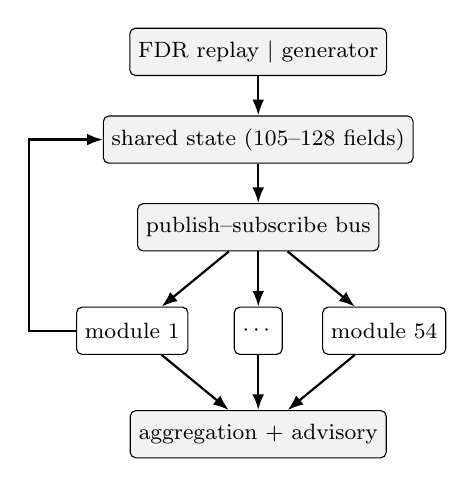
\begin{tikzpicture}[
  node distance=5mm,
  box/.style={draw, rounded corners=2pt, align=center, font=\footnotesize,
              minimum height=6mm, inner sep=3pt},
  ar/.style={-{Latex[length=2mm]}, thick}
]
\node[box, fill=black!5] (src) {FDR replay \textbar{} generator};
\node[box, fill=black!5, below=of src] (state) {shared state (105--128 fields)};
\node[box, fill=black!5, below=of state] (bus) {publish--subscribe bus};
\node[box, below=7mm of bus, xshift=-16mm] (m1) {module 1};
\node[box, below=7mm of bus] (m2) {$\cdots$};
\node[box, below=7mm of bus, xshift=16mm] (m3) {module 54};
\node[box, fill=black!5, below=7mm of m2] (agg) {aggregation + advisory};
\draw[ar] (src) -- (state);
\draw[ar] (state) -- (bus);
\draw[ar] (bus) -- (m1);
\draw[ar] (bus) -- (m2);
\draw[ar] (bus) -- (m3);
\draw[ar] (m1) -- (agg);
\draw[ar] (m2) -- (agg);
\draw[ar] (m3) -- (agg);
\draw[ar] (m1.west) -- ++(-6mm,0) |- (state.west);
\end{tikzpicture}
\caption{Event flow. The left-hand return path is the blackboard coupling
measured in Section~\ref{sec:coupling}: modules deposit derived values into
the same state other modules read.}
\label{fig:flow}
\end{figure}

\subsection{Module population}

Fifty-four detection modules span eleven operational domains
(Table~\ref{tab:domains}). Every module's alerting logic is a fixed arithmetic
function of explicit numeric thresholds rather than a learned parameter; no
module contains a trained model, and in that sense every alert is traceable to
the inputs and the rule that produced it. The thresholds are intended to
express published operating limits---ICAO Annex~6~\cite{icao_annex6}, FAR
Part~25~\cite{far25} and Part~23~\cite{far23}, published ground-proximity
warning criteria~\cite{gpws_criteria}. Section~\ref{sec:provenance} measures
how far that intent is actually documented in the code, and the answer is a
substantial qualification of it.

Two further subscribers run downstream: an aggregation stage that groups
active alerts into per-subsystem health scores, and a diversion-advisory stage
that ranks candidate airports.

\begin{table}[t]
\caption{Operational Domains}
\label{tab:domains}
\centering
\footnotesize
\begin{tabular}{@{}lrp{0.42\columnwidth}@{}}
\toprule
\textbf{Domain} & \textbf{Mods} & \textbf{Representative check} \\
\midrule
Air data / altimetry & 11 & dual-channel disagreement, baro setting \\
Engine & 7 & EGT exceedance, N1 disagreement, thrust asymmetry \\
Speed & 6 & VMO/MMO, flap and gear placard speeds \\
GPWS / terrain & 6 & sink rate, terrain closure \\
Glide / descent & 6 & glide range, VREF on final \\
Attitude & 6 & bank, pitch, sustained-$g$ \\
Approach & 6 & stabilised-approach criteria, crosswind, tailwind \\
Fuel & 5 & leak detection, endurance, diversion reserve \\
Pressurisation & 4 & cabin rate, differential, rapid decompression \\
Performance & 4 & density altitude, cruise ceiling \\
Icing & 4 & accretion rate, icing conditions \\
\bottomrule
\end{tabular}
\end{table}

\section{Method}
\label{sec:method}

All measurements were taken on a single commodity workstation
(Windows~11, CPython~3.14) replaying NASA DASHlink \emph{Sample Flight Data}
\cite{dashlink}: de-identified FDR recordings from one type of regional jet in
commercial service, 186 channels sampled at mixed rates between 0.25\,Hz and
16\,Hz. Replay runs at the recording's native base rate of 16\,Hz, giving a
real-time budget of 62.5\,ms per tick. Timing excludes file parsing and the
WebSocket transport, isolating the bus and the module population.

Cost measurements (Section~\ref{sec:cost}) instrument each subscriber
individually over 20{,}000 consecutive ticks beginning 600\,s into a
150.8-minute flight. Determinism and coupling measurements
(Section~\ref{sec:coupling}) replay identical flights repeatedly and compare
the emitted event sequences exactly. False-positive measurements
(Section~\ref{sec:validation}) run complete gate-to-gate flights. Scripts and
raw result files accompany the paper; see Data Availability.

\section{The Cost of the Decomposition}
\label{sec:cost}

\subsection{An attempted scaling law, and why it failed}

The obvious experiment is to time the bus with the first $n$ subscribers
attached and fit a line. We ran it for $n \in \{1,5,10,20,30,40,50,54\}$ over
6{,}000 ticks per point, and report it as a negative result. Mean per-tick
cost went 0.089, 0.174, 0.241, 0.218, 0.258, 0.283, 0.205 and 0.180\,ms
respectively: not monotonic, and fifty-four modules measured \emph{cheaper}
than ten. A least-squares fit returns 1.2\,$\mu$s per module on a 174\,$\mu$s
intercept with $R^2 = 0.17$, which is to say no relationship at all.

The reason is that the module population is not homogeneous, so a prefix of
the registration list is not a scaled-down copy of the whole. Different
prefixes contain different modules; because per-module cost spans more than an
order of magnitude (below), the variation \emph{between} modules swamps the
variation \emph{with count}. Most modules also gate on flight phase and return
immediately outside it, so which phase the sample window falls in matters as
much as how many modules are attached.

We report this because the previous version of this work claimed linear
scaling on exactly this basis. A prefix fit of this kind measures the
registration order, not the architecture, and we could have published the
number without noticing. The diagnostic that exposed it was instrumenting
subscribers individually rather than in aggregate.

\subsection{Per-module cost}

The informative measurement is the distribution. Table~\ref{tab:cost} gives
per-subscriber cost per tick over 20{,}000 ticks.

\begin{table}[t]
\caption{Per-Subscriber Cost Per Tick ($\mu$s), 20{,}000 Ticks at 16\,Hz}
\label{tab:cost}
\centering
\footnotesize
\begin{tabular}{@{}lrrr@{}}
\toprule
\textbf{Subscriber} & \textbf{Mean} & \textbf{p99} & \textbf{Max} \\
\midrule
\multicolumn{4}{@{}l}{\emph{Detection layer (54 modules)}} \\
\quad minimum module        & 1.16   & --      & -- \\
\quad median module         & 2.70   & --      & -- \\
\quad mean module           & 5.25   & --      & -- \\
\quad most expensive module & 65.82  & 158.4   & 4{,}208.6 \\
\quad \textbf{all 54 combined} & \textbf{283.6} & -- & -- \\
\midrule
\multicolumn{4}{@{}l}{\emph{Downstream stages (2)}} \\
\quad aggregation           & 38.0   & 87.3    & 3{,}092.9 \\
\quad diversion advisory    & 2{,}019.4 & 2{,}903.0 & 529{,}505.4 \\
\quad \textbf{both combined} & \textbf{2{,}057.4} & -- & -- \\
\bottomrule
\end{tabular}
\end{table}

Three things follow. The detection layer is cheap in absolute terms: all
fifty-four modules together consume 283.6\,$\mu$s, or 0.45\% of the 62.5\,ms
budget. Its cost is dominated by module bodies rather than by bus overhead,
and the distribution is heavily skewed---a median module costs 2.7\,$\mu$s
while the most expensive costs 65.8\,$\mu$s, a 24$\times$ spread---so
population size is a poor predictor of cost and module content is a good one.

Second, and contrary to what a modular design would predict, the cost is not
in the modules. The two downstream stages cost 2{,}057\,$\mu$s per tick
between them, 7.3$\times$ the entire fifty-four-module detection layer, almost
all of it in the diversion advisory. Adding detection modules is close to
free; the aggregation the architecture exists to enable is not.

\subsection{Meeting the deadline}

Whole-tick latency is 1.50\,ms at p50 and 4.50\,ms at p99 against a 62.5\,ms
budget. The maximum observed tick was 530\,ms---8.5$\times$ the budget---and
81 of 20{,}000 ticks (0.405\%) exceeded it. Every overrun traced to the
diversion-advisory stage performing a candidate-airport search. The system is
therefore comfortably real-time in the common case and not hard real-time at
all: it has no mechanism to bound the worst case, and the tail is produced by
a single unbounded subscriber rather than by load.

\subsection{Throughput, CPU and memory}

Run unpaced, the pipeline consumes 860 ticks/s, or 54$\times$ the recording's
16\,Hz rate: a 150-minute flight replays through all fifty-six subscribers in
under three minutes. Paced at the native rate, CPU time is 1.11\,ms per tick,
which is 1.78\% of one core. Both figures are dominated by the two downstream
stages in the same proportion as Table~\ref{tab:cost}.

Resident memory is 63\,MB for the interpreter, rising to 119\,MB once the
modules are constructed and one flight is parsed---the flight file itself,
186 channels held as dense arrays, accounts for most of that. Over 20{,}000
subsequent ticks resident memory grew by 0.3\,MB, so the rolling buffers the
modules maintain are bounded in practice as well as in intent. Peak working
set was 139\,MB.

Two caveats on these numbers. They are single-process figures on one machine
with a CPython interpreter, so they bound nothing and transfer to no other
platform. And they describe fifty-six subscribers: we have not measured a
population of several hundred, so the claim that maintenance and runtime cost
stay flat at that scale is not one this paper is in a position to make. What
the measurements do support is narrower---that at the current population the
detection layer is not the constraint, and that the first thing to become one
is the aggregation stage rather than the module count.

\section{Fault Containment}
\label{sec:containment}

A claimed benefit of the decomposition is that a misbehaving module cannot
take the system down. We tested it by attaching two deliberately faulty
subscribers: one that raises on every tick, and one that awaits for 50\,ms.

Containment of \emph{exceptions} holds. With a module raising on every tick,
all 300 test ticks completed, the remaining modules continued to evaluate, and
alerts continued to be produced; the bus catches per-subscriber exceptions and
reports them without propagating.

Containment of \emph{latency} does not hold. The concurrent fan-out completes
only when its slowest subscriber completes, so the 50\,ms module raised median
whole-tick latency from 1.50\,ms to 62.56\,ms---at the deadline, from a single
subscriber, with the other fifty-five modules idle and waiting.

The word ``concurrent'' is doing misleading work in the original description of
this design, and the distinction matters. The fan-out is concurrent in the
sense that subscribers are dispatched together and may interleave at await
points; it is not parallel, and it offers no preemption. A subscriber that
blocks, loops, or awaits a slow resource holds the tick, and nothing in the
architecture can take it back. Adding modules more carefully does not help,
because the property being violated is not a property of any module.

Two mitigations are standard and neither is present. Per-subscriber timeouts
would bound the damage at the cost of dropping that module's evaluation for
the tick, which for a monitor means deciding which checks may be skipped under
load---a safety argument, not an engineering convenience. Time and space
partitioning of the kind ARINC~653~\cite{arinc653} specifies for integrated
modular avionics bounds it properly, by construction, and is the reason that
standard exists.

A related hazard raised in review is priority inversion, and it takes an
unusual form here. Because there are no priorities---every subscriber is
dispatched with equal standing and runs to completion---a low-criticality
subscriber cannot be preempted by a high-criticality one, so the
diversion-advisory search delays a stall or terrain check just as readily as
it delays an advisory. The system does not suffer priority inversion so much
as it forgoes priority altogether, which is the weaker position of the two: a
scheduler that inverts priority at least represents criticality and can be
fixed, whereas this one has no representation of criticality to fix. Any
serious version of this design would need alert criticality to be a
first-class scheduling property rather than a field in the emitted event. The measurement here is best read as a demonstration of what
a monitoring architecture without partitioning gives up: the observed 0.4\%
deadline-miss rate of Section~\ref{sec:cost} arises from an ordinary
subscriber doing ordinary work, with no faulty module involved at all.

\section{Determinism and Shared-State Coupling}
\label{sec:coupling}

\subsection{Why a data race cannot occur}

Reviewers of the earlier version raised concurrent read/write hazards on the
shared state. The question deserves a precise answer rather than a
reassurance. The fan-out dispatches all subscribers with a single
\texttt{gather} on one event loop in one OS thread. Scheduling is cooperative,
not preemptive: a handler runs uninterrupted until it awaits, and suspended
tasks resume in a deterministic FIFO order. There is no preemption and no
parallelism, so two handlers cannot interleave mid-statement and a data race
in the conventional sense is impossible.

We verified this empirically rather than resting on the argument. Replaying an
identical flight five times produced byte-identical alert sequences. Because a
non-yielding event sink would make that trivially true, we repeated it with a
sink that yields on every emission, as a real socket write does: the sequences
remained identical.

\subsection{The hazard that is real}

Determinism is not correctness. A static audit of the fifty-five state
handlers found \textbf{eleven} that reach an \texttt{await} before finishing
their writes to the shared state---exactly the pattern under which a
successor module can observe a partially-updated state. It is deterministic,
and it can still be wrong.

Table~\ref{tab:coupling} measures the exposure. The shared state carries
nineteen derived fields written by modules for other modules to read. Fifteen
are read only by the module that wrote them, and are therefore private in
effect if not in form. Four cross a module boundary, and those four are the
entire coupling surface of a fifty-four-module population.

\begin{table}[t]
\caption{Shared-State Coupling Surface}
\label{tab:coupling}
\centering
\footnotesize
\begin{tabular}{@{}lrl@{}}
\toprule
\textbf{Derived field} & \textbf{Ext.\ readers} & \textbf{Consumer} \\
\midrule
\texttt{glideslope\_dots} & 3 & go-around, unstable approach \\
\texttt{crosswind\_kts}   & 1 & go-around advisory \\
\texttt{tailwind\_kts}    & 1 & go-around advisory \\
\texttt{assessment}       & 1 & diversion advisory \\
\midrule
15 further derived fields & 0 & written and read by one module \\
\bottomrule
\end{tabular}
\end{table}

Every producer happens to be registered before its consumer, so consumers see
the current tick's values. Nothing enforces this. Permuting the subscriber
order changed the emitted event sequence while leaving per-alert-type counts
unchanged on the flight tested, confirming the dependency is live rather than
theoretical.

The failure mode deserves emphasis because it is the wrong way round. The
consumers read with a default: \texttt{state.get("crosswind\_kts", 0.0)}. Zero
is inside every limit these modules test. A consumer that runs before its
producer therefore does not fail loudly or raise a spurious alert---it
silently substitutes a value that cannot trigger anything, and the alert is
\emph{suppressed}. A registration-order mistake in a monitoring system thus
manifests as a missing warning, which is the failure direction that matters
most and the one least likely to be noticed in test.

\section{Validation Against Recorded Flight Data}
\label{sec:validation}

\subsection{From a generated state to a recorded one}

During development the shared state was populated by a parametric flight-state
generator producing a plausible gate-to-gate flight at a fixed 30\,Hz. An
earlier formulation treated the provenance of the state as orthogonal to the
architecture, since the bus and the module contract constrain only the
\emph{shape} of the state.

Driving the same unmodified module population with recorded FDR data tested
that. The architectural half of the claim held: substituting the source
required no change to the bus, the module contract, the event schema or the
aggregation stage---a replay adapter mapping recorded channels onto
shared-state field names was sufficient. The module population did not hold. A
single \emph{normal} flight, containing no emergency of any kind, produced
2{,}409 alert transitions.

\subsection{Four classes of concealed defect}

Diagnosis attributed the spurious annunciations to four classes, each
invisible to a synthetic source because the generator, written by the same
author as the modules, shared their assumptions.

\textit{Sentinel encodings read as measurements.} Recorders emit fixed
out-of-range values to mark dropped samples rather than leaving gaps. Vertical
acceleration parks at exactly $-3.375$\,g for 2.8\% of a normal flight; oil
temperature parks at $-390$\,$^\circ$C. Read as readings, the acceleration
sentinel alone produced 1{,}635 phantom negative-$g$ events---the single
largest contributor, and by itself two-thirds of the total. The generator
never emitted a dropout, so no module had ever needed to distinguish a marker
from a measurement, and nothing in the state contract carried the information
that would let one. The repair was a per-channel plausible-range filter with a
last-good hold, applied in the replay adapter rather than in the modules.

\textit{Time-base errors masked by a fixed rate.} Several modules divided
accumulated change by a tick count rather than by elapsed time. At the
generator's fixed 30\,Hz the two are proportional and the constant folds
silently into whatever threshold was tuned against it; at 16\,Hz they are not.
Two modules computing terrain-closure and cabin-decompression rates were
understating them by the ratio of the rates, which rendered both effectively
inert---a defect that produces no spurious alert and therefore shows up in no
false-positive count. It is visible only by changing the sample rate, which a
fixed-rate generator by construction cannot do. This class argues for
exercising a monitor at more than one rate regardless of what rate it will
eventually run at.

\textit{Thresholds without hysteresis.} Real channels are quantised---airspeed
to 0.25\,kt at 4\,Hz---so a signal resting near a limit does not approach it
smoothly but steps across it repeatedly. The overspeed module produced 216
transitions on a flight with no genuine exceedance. Gaussian generator noise,
being continuous and zero-mean, averages out over a short smoothing window in
a way quantisation does not: at 4\,Hz a one-second window holds four samples,
and a single quantisation step across that window reads as a 1\,kt/s trend.
The repair was an asymmetric latch---immediate escalation for critical
conditions, a dwell requirement for cautions and for clears---rather than a
wider threshold, which would have traded the chatter for lost sensitivity.

\textit{Parameter provenance.} The most consequential class. Modules compared
recorded values against limits for the wrong airframe, and in one case
confused an observed-typical value with a certified limit: a reference landing
speed derived as the median of observed finals is by construction a value the
aircraft is below half the time. Correcting the approach-speed module required
identifying the airframe class from its own recorded maximum-operating-speed
channel and gating the check at 1{,}000\,ft above ground rather than 3{,}000\,ft
above sea level, matching stabilised-approach criteria. That single correction
took the module from 48 spurious alerts to zero.

\subsection{Result}

Table~\ref{tab:defects} attributes the baseline count and reports the current
measured figure. We note explicitly that the baseline and the corrected figure
are measured; the attribution of intermediate counts to individual corrections
is by alert identifier and does not constitute a measured time series of
successive builds.

\begin{table}[t]
\caption{Spurious Annunciations, One Normal Recorded Flight}
\label{tab:defects}
\centering
\footnotesize
\begin{tabular}{@{}lrr@{}}
\toprule
\textbf{Defect class} & \textbf{Attributed} & \textbf{After} \\
\midrule
Sentinel read as measurement & 1{,}635 & 0 \\
Threshold chatter (no hysteresis) & 216 & 0 \\
Parameter provenance (approach speed) & 48 & 0 \\
Time-base errors and remainder & 510 & -- \\
\midrule
\textbf{Total, before correction} & \textbf{2{,}409} & \\
\textbf{Total, after correction} & & \textbf{33} \\
\bottomrule
\end{tabular}
\end{table}

Re-measured on the current implementation over the complete 150.8-minute
flight (144{,}768 ticks), the same flight now raises 33 alerts, a rate of
13.1 per flight hour. The largest remaining contributors are terrain-closure
(10) and glide-range (4) advisories, which are plausible on a short-sector
regional operation and have not been separately adjudicated against the
recording.

\subsection{Provenance of the encoded limits}
\label{sec:provenance}

The fourth defect class raises a question the previous version of this work did
not ask: if modules encode published limits, how is that encoding verified? We
audited it. Across the fifty-four detection modules there are 133 module- and
class-level numeric constants. Seven modules (13\%) name a regulatory source
anywhere in their text---four ICAO, two FAR Part 25, one an aircraft manual.
Forty-seven modules, holding 113 of the 133 constants, name no source at all.

No constant is checked against its document by anything automated, and a named
source in a comment is not a machine-checkable claim. The honest description
is therefore that the limits were \emph{sourced} by the author during
development and are \emph{documented} for one module in eight. The earlier
statement that module logic is ``a fixed function of named published limits''
is accurate about the \emph{form} of the logic and overstates the state of its
\emph{provenance}; we correct it here.

This matters more than a documentation gap because the fourth defect class is
what an unverified constant looks like in operation. A reference landing speed
derived as the median of observed finals is not a limit at all---it is a value
the aircraft is below half the time---and nothing in the code distinguished it
from a certified one. The audit therefore measures the surface on which that
class of defect can recur: 113 constants with no recorded origin.

We also record, in answer to the same question, that the system has no
automated test suite. There are no unit tests over module logic, no golden
traces, and no regression harness; the measurement scripts accompanying this
paper are the only executable checks in the repository. Every correctness
claim in Section~\ref{sec:validation} rests on differential comparison of
alert counts between builds, which detects changes in aggregate behaviour and
would not detect a module that is wrong in the same way before and after.

\subsection{Interpretation}

The architectural claim and the module-population claim came apart. The
architecture absorbed a complete change of data provenance without
modification, and every defect was repaired inside a single module without
touching the bus, the schema or any other module. That containment is the
decomposition's real payoff and it is worth stating plainly.

But the same result refines the orthogonality claim rather than confirming it.
A contract that constrains only the \emph{shape} of the state necessarily
leaves every assumption about its \emph{meaning}---units, sample rate, sentinel
encoding, which airframe a constant belongs to---inside the modules, where the
contract cannot see them. Modularity did not remove those assumptions; it
relocated them, and made them cheap to fix once found. Finding them required a
data source the module authors did not write.

\section{Threats to Validity}
\label{sec:threats}

\textit{Single platform.} All timings come from one workstation and one
Python implementation. Absolute figures will not transfer; the ratio between
the detection layer and the downstream stages, which is the load-bearing
result, is less sensitive to platform.

\textit{Single airframe type.} The corpus covers one regional-jet type. The
provenance findings concern the relationship between a module's constants and
the airframe producing the data, and would be expected to recur---differently
---on any other type.

\textit{No genuine emergencies.} The corpus records routine operations. Every
alert counted is therefore a false positive or a genuine exceedance the crew
flew through, and the study measures false-positive behaviour only. It
establishes nothing about detection sensitivity, and the two-order-of-magnitude
reduction reported above must be read with that limitation in view: a monitor
that never alerts would score perfectly on this metric.

\textit{Author-diagnosed defects.} The four defect classes were identified by
the system's own author, who also wrote both the modules and the generator
that concealed the defects. The classification is therefore a structured
account of one debugging effort, not an independently validated taxonomy, and
a different author pairing might have produced a different set. What the
result does establish is weaker and still useful: that a generator written by
the module author can hide defects of these kinds for an entire development
cycle.

\textit{Extension cost is not measured.} A previous version reported the number
of files modified to add a module as evidence of constant-cost extension. That
table is withdrawn. The figure is true by construction of the composition-root
pattern rather than by experiment, it would hold for any single addition to
any such system, and it says nothing about whether the cost stays flat as a
population grows. Measuring extension cost properly would require adding many
modules over time and tracking the effort, which we have not done.

\section{Limitations}
\label{sec:limits}

\textit{No certification argument is made.} An earlier version suggested that
the composition root allows modules to be added without re-validating the
system. That claim is withdrawn. Under DO-178C~\cite{do178c}, modifying shared
data, altering a composition root, or changing memory and execution load all
require impact analysis, regression verification and evidence of
non-interference, at a rigour set by the design assurance level. Nothing in
this paper constitutes such evidence, and the system is a research artifact,
not airborne software.

\textit{Contracts are conventions.} The module contract and event schema are
enforced by developer discipline, not by types, schemas or static checks. The
eleven handlers identified in Section~\ref{sec:coupling} are the measurable
cost of that choice, and the defect classes of Section~\ref{sec:validation}
are its consequences.

Three of the four classes are mechanically preventable by a state contract
that declares, per field, a unit, a plausible range, a sample rate and a
validity predicate. A declared range turns the $-3.375$\,g sentinel into a
rejected sample at the boundary rather than a reading inside a module. A
declared rate removes the temptation to divide by a tick count, because
elapsed time becomes available from the field itself. A declared unit makes
the airframe-provenance mismatch a type error rather than a plausible number.
Only the observed-typical-versus-certified-limit confusion survives, because
that is a question about where a constant came from rather than about what it
means---which suggests constants should carry a cited source as metadata, not
merely a comment. We regard this as the most valuable single extension
available to the system and have not implemented it.

\textit{Aggregation is not principled fusion.} The health stage applies fixed
deductions per active alert. This is arithmetic, not evidence combination: it
has no model of sensor reliability, no treatment of conflicting or correlated
evidence, and no way to represent a cascade in which one root cause produces
many alerts. Dempster--Shafer evidence theory~\cite{shafer1976}, widely applied
to multi-sensor fault diagnosis~\cite{ds_survey2022}, and Bayesian or
fault-tree formulations, are the established alternatives. Replacing the
deduction scheme is future work and we make no claim for the present scheme
beyond transparency.

\textit{Naive evaluation strategy.} Every module is re-evaluated every tick.
Section~\ref{sec:cost} shows this is affordable at fifty-four modules, but a
RETE-style incremental match~\cite{forgy1982} would be the correct answer at a
population where it is not.

\section{Conclusion}

We measured a fifty-four-module rule-based aircraft health monitor on recorded
FDR data, having first withdrawn the claim that its architecture was novel. The
decomposition is affordable---0.45\% of the real-time budget for the whole
detection layer, a median module costing 2.7\,$\mu$s---and it contains
exceptions and localises defects effectively: every one of four classes of
provenance defect was repaired inside a single module.

It also fails in ways a modular design does not advertise. The cost is
concentrated in the aggregation stage, not the modules, at 7.3$\times$ the
detection layer, and that stage drives a 0.4\% deadline-miss rate with an
unbounded tail. Latency is not contained at all: one slow subscriber consumes
the whole budget. And the shared state, though free of data races under
cooperative scheduling, carries four cross-module dependencies whose ordering
is unenforced and whose failure mode is a suppressed alert.

The general observation is that modular decomposition relocates assumptions
rather than eliminating them. A contract over the shape of a shared state
cannot constrain the meaning of what flows through it, so meaning-level
assumptions accumulate precisely at the architecture--module boundary, where
they are invisible to the contract and visible only to a data source the module
authors did not write.

\section*{Data Availability and Acknowledgment}

Flight data are from NASA's DASHlink \emph{Sample Flight Data} corpus
\cite{dashlink}, released for research use; the authors of this paper are not
affiliated with NASA and the data are used as distributed. The OpenSky
in-flight-emergency reference dataset~\cite{olive_zenodo,olive2020}, built on
the OpenSky Network~\cite{schafer2014} using the \texttt{traffic} library
\cite{olive2019}, is acknowledged as the intended source for future work on
genuine emergency trajectories; it is distributed under a non-commercial
licence. Measurement scripts and raw result files supporting
Sections~\ref{sec:cost}--\ref{sec:validation} are available from the author.

\begin{thebibliography}{00}

\bibitem{cugola2012}
G. Cugola and A. Margara, ``Processing flows of information: From data stream
to complex event processing,'' \emph{ACM Computing Surveys}, vol.~44, no.~3,
article~15, 2012.

\bibitem{forgy1982}
C. L. Forgy, ``Rete: A fast algorithm for the many pattern/many object pattern
match problem,'' \emph{Artificial Intelligence}, vol.~19, no.~1, pp.~17--37,
1982.

\bibitem{iso13374}
International Organization for Standardization, ``Condition monitoring and
diagnostics of machines---Data processing, communication and
presentation---Part 1: General guidelines,'' ISO 13374-1, 2003.

\bibitem{nii1986}
H. P. Nii, ``Blackboard systems: The blackboard model of problem solving and
the evolution of blackboard architectures,'' \emph{AI Magazine}, vol.~7,
no.~2, pp.~38--53, 1986.

\bibitem{buschmann1996}
F. Buschmann, R. Meunier, H. Rohnert, P. Sommerlad, and M. Stal,
\emph{Pattern-Oriented Software Architecture: A System of Patterns}.
Chichester, U.K.: Wiley, 1996.

\bibitem{hohpe2003}
G. Hohpe and B. Woolf, \emph{Enterprise Integration Patterns}. Boston, MA:
Addison-Wesley, 2003.

\bibitem{do178c}
RTCA, ``Software considerations in airborne systems and equipment
certification,'' RTCA DO-178C, 2011.

\bibitem{arinc653}
Aeronautical Radio, Inc., ``Avionics application software standard
interface,'' ARINC Specification 653, 2019.

\bibitem{shafer1976}
G. Shafer, \emph{A Mathematical Theory of Evidence}. Princeton, NJ: Princeton
University Press, 1976.

\bibitem{ds_survey2022}
F. Xiao, ``A survey: Optimization and applications of evidence fusion
algorithm based on Dempster--Shafer theory,'' \emph{Applied Soft Computing},
vol.~124, 109075, 2022.

\bibitem{icao_annex6}
International Civil Aviation Organization, \emph{Annex 6 to the Convention on
International Civil Aviation: Operation of Aircraft}, Part I, 11th ed.
Montreal, Canada: ICAO, 2018.

\bibitem{far25}
U.S. Federal Aviation Administration, ``Airworthiness standards: Transport
category airplanes,'' 14 CFR Part 25.

\bibitem{far23}
U.S. Federal Aviation Administration, ``Airworthiness standards: Normal
category airplanes,'' 14 CFR Part 23.

\bibitem{gpws_criteria}
U.S. Federal Aviation Administration, ``Terrain awareness and warning system
(TAWS),'' Technical Standard Order TSO-C151, 2012.

\bibitem{dunsdon2008}
J. Dunsdon and M. Harrington, ``The application of open system architecture
for condition based maintenance to complete IVHM,'' in \emph{Proc. IEEE
Aerospace Conf.}, 2008, pp.~1--9.

\bibitem{bahon2007}
C. Bahon, ``Integrated vehicle health management: The technology,'' in
\emph{Proc. SAE Aerospace Technology Conf.}, 2007.

\bibitem{li2022}
R. Li, W. J. C. Verhagen, and R. Curran, ``A systematic methodology for
prognostic and health management system architecture definition,''
\emph{Reliability Engineering \& System Safety}, vol.~193, 106598, 2020.

\bibitem{denecke2011}
C. Denecke, ``Aircraft health monitoring: Concepts and architectures,'' in
\emph{Proc. Deutscher Luft- und Raumfahrtkongress}, 2011.

\bibitem{bisanti2023}
G. M. Bisanti, G. Mainetti, L. Patrono, and I. Sergi, ``Digital technologies
for aircraft health monitoring: A systematic review,'' in \emph{Proc. Int.
Conf. Software, Telecommunications and Computer Networks}, 2023.

\bibitem{kabashkin2024}
I. Kabashkin, B. Misnevs, and O. Zervina, ``Artificial intelligence in
aviation: New professionals for new technologies,'' \emph{Applied Sciences},
vol.~13, no.~21, 11660, 2023.

\bibitem{dashlink}
NASA Ames Research Center, ``DASHlink: Sample flight data,'' NASA Aviation
Safety Program. [Online]. Available: https://c3.ndc.nasa.gov/dashlink/

\bibitem{matthews2013}
B. L. Matthews, S. Das, K. Bhaduri, K. Das, R. Martin, and N. Oza,
``Discovering anomalous aviation safety events using scalable data mining
algorithms,'' \emph{Journal of Aerospace Information Systems}, vol.~10,
no.~10, pp.~467--475, 2013.

\bibitem{olive2020}
X. Olive, M. Strohmeier, and J. L\"ubbe, ``Reference datasets for in-flight
emergency situations,'' in \emph{Proc. 8th OpenSky Symposium}, 2020.

\bibitem{olive_zenodo}
X. Olive, M. Strohmeier, and J. L\"ubbe, ``Crowdsourced air traffic data from
the OpenSky Network 2019--2020,'' Zenodo, 2020,
doi:10.5281/zenodo.3937483.

\bibitem{schafer2014}
M. Sch\"afer, M. Strohmeier, V. Lenders, I. Martinovic, and M. Wilhelm,
``Bringing up OpenSky: A large-scale ADS-B sensor network for research,'' in
\emph{Proc. ACM/IEEE Int. Conf. Information Processing in Sensor Networks},
2014, pp.~83--94.

\bibitem{olive2019}
X. Olive, ``traffic, a toolbox for processing and analysing air traffic
data,'' \emph{Journal of Open Source Software}, vol.~4, no.~39, 1518, 2019.

\end{thebibliography}

\end{document}
